

\tikzset{every picture/.style={line width=0.75pt}} %set default line width to 0.75pt        

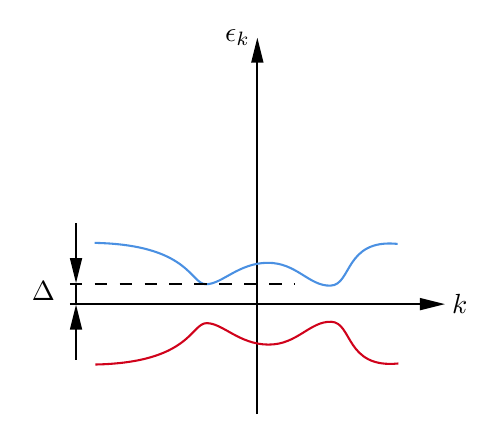
\begin{tikzpicture}[x=0.75pt,y=0.75pt,yscale=-1,xscale=1]
%uncomment if require: \path (0,300); %set diagram left start at 0, and has height of 300

%Straight Lines [id:da3923768503429792] 
\draw    (93,198) -- (271.71,198) ;
\draw [shift={(273.71,198)}, rotate = 180] [fill={rgb, 255:red, 0; green, 0; blue, 0 }  ][line width=0.08]  [draw opacity=0] (12,-3) -- (0,0) -- (12,3) -- cycle    ;
%Straight Lines [id:da007460559717310078] 
\draw    (183.35,251) -- (183.35,71.69) ;
\draw [shift={(183.35,69.69)}, rotate = 450] [fill={rgb, 255:red, 0; green, 0; blue, 0 }  ][line width=0.08]  [draw opacity=0] (12,-3) -- (0,0) -- (12,3) -- cycle    ;
%Curve Lines [id:da5016211924753684] 
\draw [color={rgb, 255:red, 74; green, 144; blue, 226 }  ,draw opacity=1 ]   (104.95,168.5) .. controls (150.96,169.43) and (150.96,188.43) .. (158.63,188.43) .. controls (166.3,188.43) and (174.27,178.19) .. (188.3,178.1) .. controls (202.32,178.01) and (208.3,189.43) .. (218.63,189.1) .. controls (228.96,188.77) and (225.3,166.43) .. (250.95,169) ;
%Curve Lines [id:da07180929244633205] 
\draw [color={rgb, 255:red, 208; green, 2; blue, 27 }  ,draw opacity=1 ]   (105.29,227.11) .. controls (151.3,226.17) and (151.3,207.17) .. (158.96,207.17) .. controls (166.63,207.17) and (174.61,217.42) .. (188.63,217.51) .. controls (202.65,217.6) and (208.63,206.17) .. (218.96,206.51) .. controls (229.3,206.84) and (225.63,229.17) .. (251.29,226.61) ;
%Straight Lines [id:da7044155195594983] 
\draw  [dash pattern={on 4.5pt off 4.5pt}]  (93,188.32) -- (201.49,188.32) ;
%Straight Lines [id:da29258181497582525] 
\draw    (96,159.04) -- (96,185.84) ;
\draw [shift={(96,187.84)}, rotate = 270] [fill={rgb, 255:red, 0; green, 0; blue, 0 }  ][line width=0.08]  [draw opacity=0] (12,-3) -- (0,0) -- (12,3) -- cycle    ;
%Straight Lines [id:da23633048347113395] 
\draw    (96,187.84) -- (96,198.27) ;
%Straight Lines [id:da5558233224671132] 
\draw    (96,200.27) -- (96,225.04) ;
\draw [shift={(96,198.27)}, rotate = 90] [fill={rgb, 255:red, 0; green, 0; blue, 0 }  ][line width=0.08]  [draw opacity=0] (12,-3) -- (0,0) -- (12,3) -- cycle    ;

% Text Node
\draw (275.71,198) node [anchor=west] [inner sep=0.75pt]    {$\boldsymbol{k}$};
% Text Node
\draw (181.35,69.69) node [anchor=east] [inner sep=0.75pt]    {$\epsilon _{\boldsymbol{k}}$};
% Text Node
\draw (73.2,185.52) node [anchor=north west][inner sep=0.75pt]    {$\Delta $};


\end{tikzpicture}
